\chapter{Applying Rapid Whole-Genome Sequencing To Predict Phenotypic Antimicrobial Susceptibility Testing Results among Carbapenem-Resistant \textit{Klebsiella pneumoniae} Clinical Isolates}
\label{chap:amr}

\textbf{Portions of this chapter originally appeared in:} \\
Tamma PD, Fan Y, Bergman Y, Pertea G, Kazmi AQ, Lewis S, et al. Applying Rapid Whole-Genome Sequencing To Predict Phenotypic Antimicrobial Susceptibility Testing Results among Carbapenem-Resistant \textit{Klebsiella pneumoniae} Clinical Isolates 2019;63. https://doi.org/10.1128/AAC.01923-18

\section{Abstract}
\label{sec:abstract}

Standard antimicrobial susceptibility testing (AST) approaches lead to delays in the selection of optimal antimicrobial therapy. Here, we sought to determine the accuracy of antimicrobial resistance (AMR) determinants identified by Nanopore whole-genome sequencing in predicting AST results. Using a cohort of 40 clinical isolates (21 carbapenemase-producing carbapenem-resistant \textit{Klebsiella pneumoniae}, 10 non-carbapenemase-producing carbapenem-resistant \textit{K. pneumoniae}, and 9 carbapenem-susceptible \textit{K. pneumoniae} isolates), three separate sequencing and analysis pipelines were performed, as follows: (i) a real-time Nanopore analysis approach identifying acquired AMR genes, (ii) an assembly-based Nanopore approach identifying acquired AMR genes and chromosomal mutations, and (iii) an approach using short-read correction of Nanopore assemblies. The short-read correction of Nanopore assemblies served as the reference standard to determine the accuracy of Nanopore sequencing results. With the real-time analysis approach, full annotation of acquired AMR genes occurred within 8 h from subcultured isolates. Assemblies sufficient for full resistance gene and single-nucleotide polymorphism annotation were available within 14 h from subcultured isolates. The overall agreement of genotypic results and anticipated AST results for the 40 \textit{K. pneumoniae} isolates was 77\% (range, 30\% to 100\%) and 92\% (range, 80\% to 100\%) for the real-time approach and the assembly approach, respectively. Evaluating the patients contributing the 40 isolates, the real-time approach and assembly approach could shorten the median time to effective antibiotic therapy by 20 h and 26 h, respectively, compared to standard AST. Nanopore sequencing offers a rapid approach to both accurately identify resistance mechanisms and to predict AST results for \textit{K. pneumoniae} isolates. Bioinformatics improvements enabling real-time alignment, coupled with rapid extraction and library preparation, will further enhance the accuracy and workflow of the Nanopore real-time approach.

\section{Introduction}
\label{sec:intro}

Whole-genome sequencing (WGS) has enabled notable advancements to the field of infectious diseases, such as an improved understanding of transmission dynamics and outbreak analysis \citep{Didelot2012-hg}. An exciting possibility from this technology is the ability to predict antimicrobial susceptibility testing (AST) results based on the identification of acquired resistance genes and/or chromosomal mutations \citep{Shelburne2017-dm}.

Currently, there are several shortcomings with standard approaches to AST, particularly as they relate to multidrug-resistant Gram-negative (MDRGN) organisms. First, AST results are reported approximately 48 to 72 h after the time of culture collection, potentially leading to delays in appropriate empirical antibiotic therapy \citep{Caliendo2013-yw}. Second, automated AST panels are limited in the number of antibiotic agents included. For agents that frequently need to be considered for highly drug-resistant pathogens (e.g., colistin, tigecycline, ceftazidime-avibactam, etc.) and newer agents in later phases of development that are unlikely to be routinely included in AST panels for the foreseeable future, there are additional delays in AST determination. As it is generally not evident at the time antibiotics are initiated that a patient will be infected with an MDRGN organism, susceptibility testing for these last-resort agents occurs subsequent to, and not simultaneously with, automated AST testing. Third, standard AST reporting does not include identification of resistance mechanisms (e.g., carbapenemases, extended-spectrum {\textbeta}-lactamases [ESBLs], etc.), which can be important for guiding antibiotic treatment decisions, as \textit{in vitro} activity does not always translate to \textit{in vivo} activity \citep{Tamma2017-el}. WGS can potentially alleviate many of these concerns by offering the potential to predict AST results by identifying the presence or absence of resistance genes, as well as mutations in relevant genes, from which clinicians can infer the activity of antibiotic agents. Furthermore, once sequencing data has been collected, it can be used to place bacterial isolates in the context of previously acquired data, which can be useful for genomic epidemiological studies and surveillance.

Oxford Nanopore Technologies (Oxford, England) has created a Nanopore-based DNA sequencer that sequences DNA by monitoring the electrical current as DNA passes through a protein pore. Unlike second-generation sequencing methods, which require the entire run to be completed before data can be analyzed, Nanopore sequencing streams long-read data in real time \citep{Cao2016-oj}, allowing for resistance gene identification within as few as 15 min of beginning the sequencing run \citep{Schmidt2017-ng, Lemon2017-td, Judge2015-zw}. As the duration of time needed for DNA extraction and library preparation techniques continues to be reduced, the total time to identification of resistance determinants from organism growth could conceivably be accomplished within a single laboratory shift. To further advance this science, we evaluated the correlation of resistance determinants identified through Nanopore sequencing with AST results in a cohort of 40 clinical \textit{Klebsiella pneumoniae} complex isolates ({\bf Figure \ref{fig:r21cartoon}}). This also enabled us to quantify the potential decrease in time to effective antibiotic therapy for the patients contributing isolates with the use of WGS using real-time analysis or rapid assembly approaches compared to that with traditional AST methods.



\begin{figure}[!ht]
\centering
\includegraphics[width = 1\linewidth,keepaspectratio]{figure/r21cartoon.pdf}
\caption[Study overview]{{\bf Study overview.} Samples were collected from patients, and bacterial isolates were cultured and identified. Isolates were then sequenced in parallel with undergoing phenotypic AST. }
\label{fig:r21cartoon}
\end{figure}


As AMR can result from plasmid-mediated gene acquisition or point mutations to drug targets ({\bf Figure \ref{fig:rescartoons}}), detecting both would be vital to predicting resistance phenotypes from genotypic data. While real-time analysis of nanopore data can enable the detection of whole genes within minutes, individual reads remain too error prone to detect small point mutations. In order to detect these, we used consensus sequences such as those generated by genome assembly must be used ({\bf Figure \ref{fig:pipeline}}). While this vastly improves sequence accuracy, most systematic errors around homopolymers and methylation motifs have been found to persist ({\bf Figure \ref{fig:npfixes}}). To address this, we further corrected the assemblies using nanopolish, which leverages the raw electrical signal produced by the sequencer to improve consensus accuracy.

\begin{figure}[!ht]
\centering
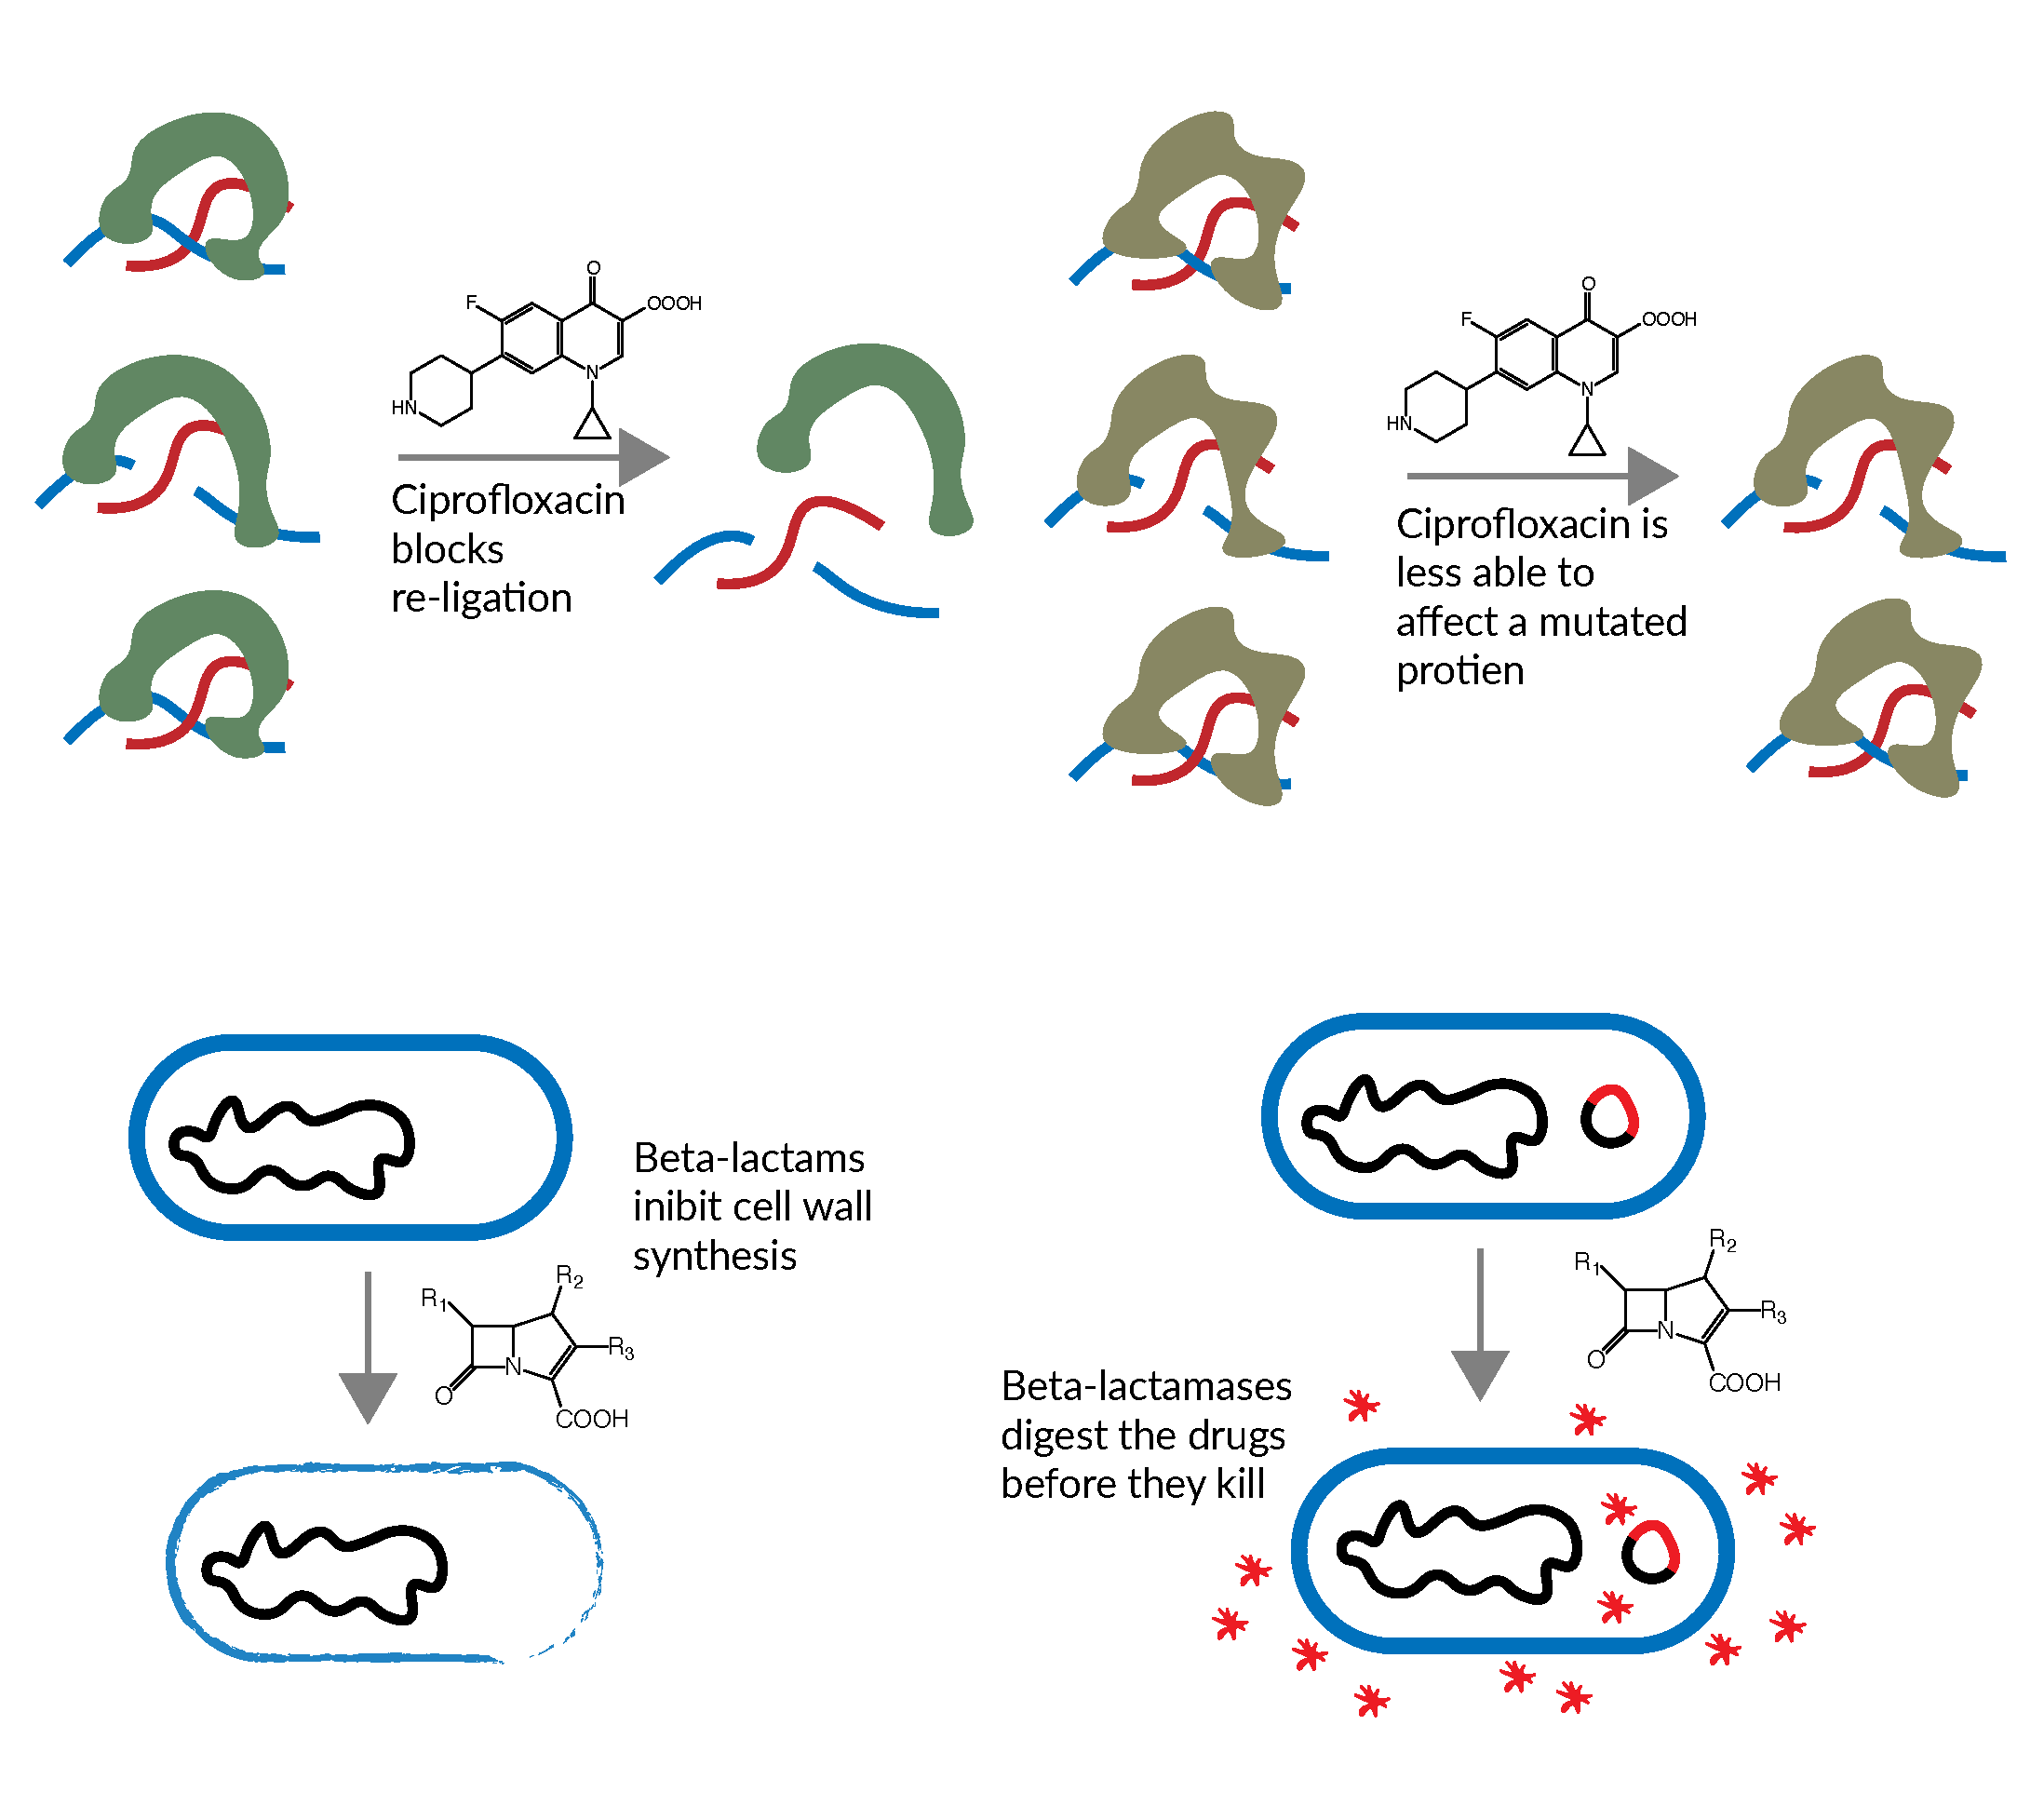
\includegraphics[width = .81\linewidth,keepaspectratio]{figure/rescartoons.pdf}
\caption[Resistance mechanisms]{{\bf Resistance mechanisms.} Drug resistances can arise through acquisition of a protective gene, such a {\textbeta}-lactamase gene. Mutations to a drug target such as the \textit{gyrA} topoisomerase gene can also reduce the effectiveness of antimicrobial agents. }
\label{fig:rescartoons}
\end{figure}


\begin{figure}[!ht]
\centering
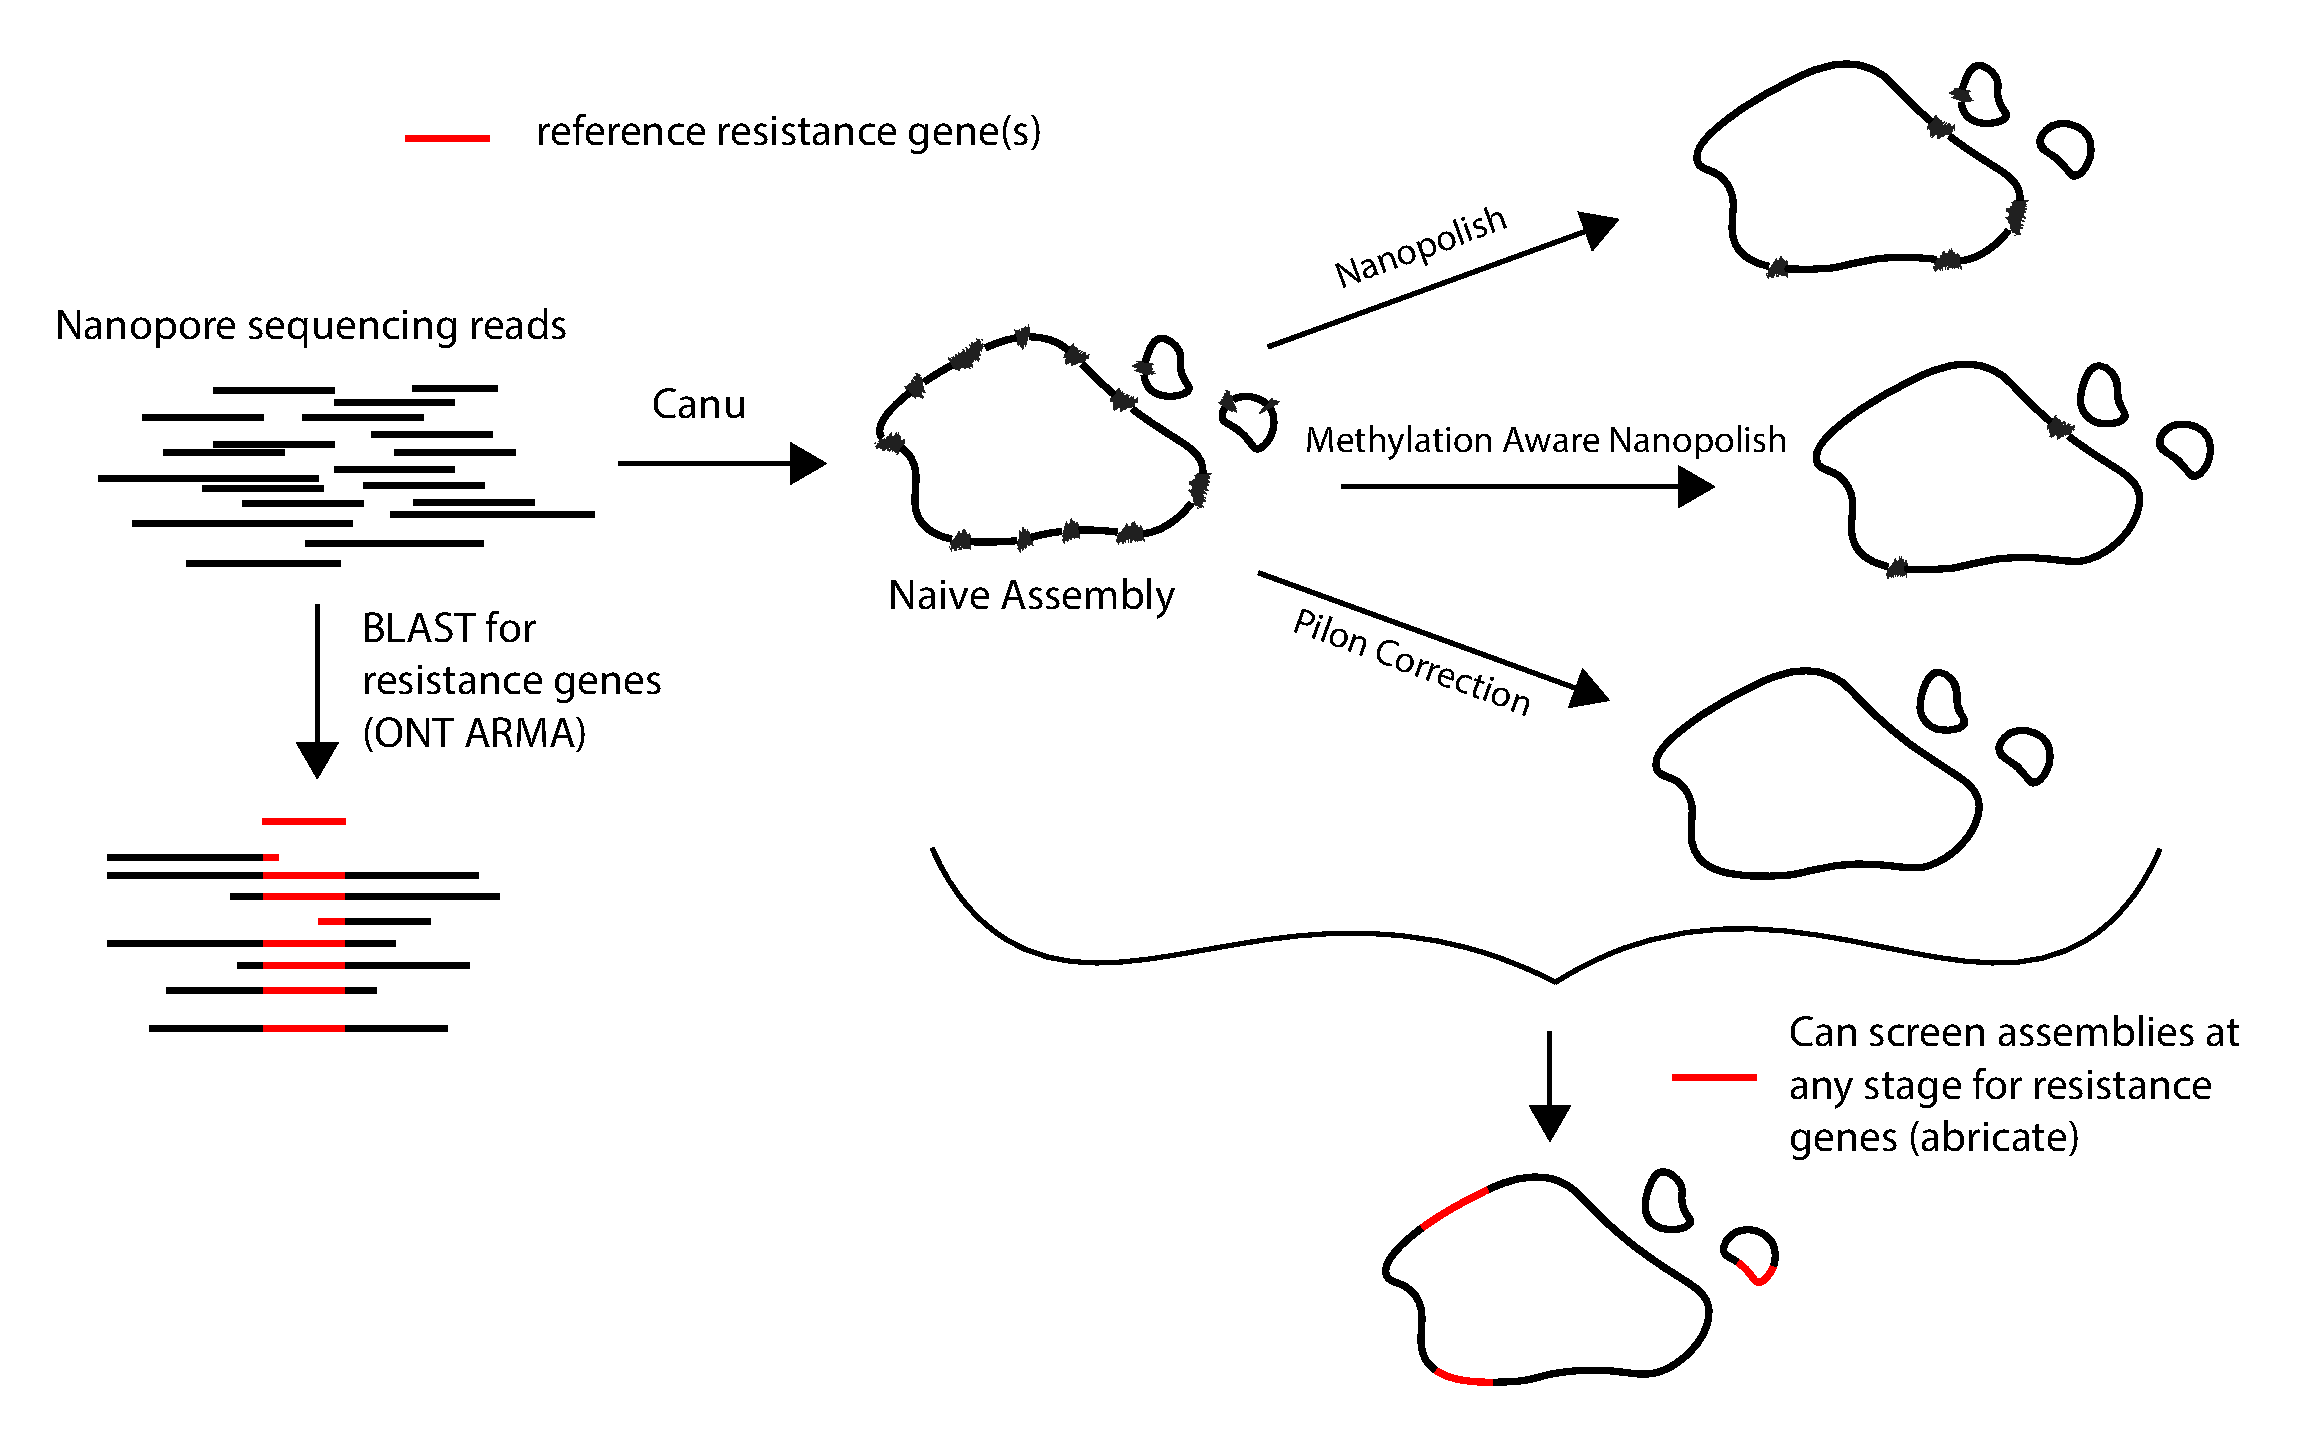
\includegraphics[width = 1\linewidth,keepaspectratio]{figure/pipeline.pdf}
\caption[Sequencing analysis pipeline]{{\bf Sequencing analysis pipeline.} Sequencing reads can be searched in real-time for resistance genes. To detect and assess point mutations, genomes are assembled, and then can be polished using native electrical data (Nanopolish), or highly accurate short-read data (Pilon). }
\label{fig:pipeline}
\end{figure}


\begin{figure}[!ht]
\centering
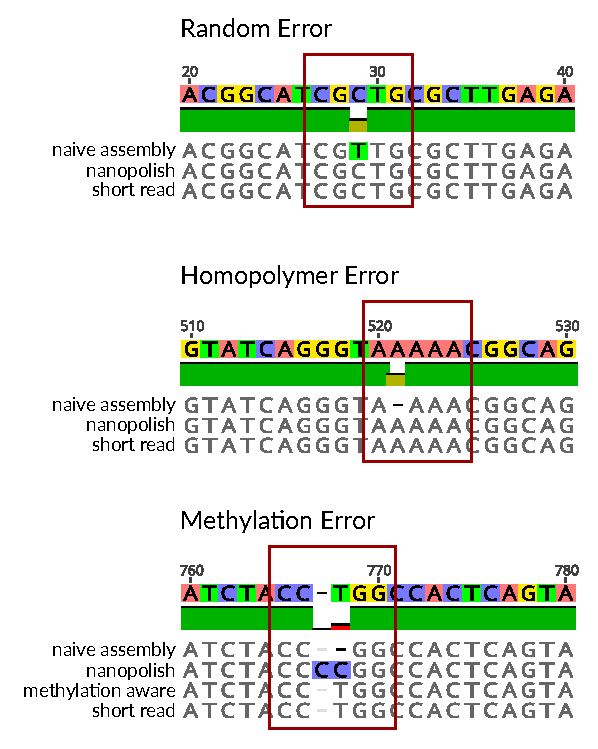
\includegraphics[width = .75\linewidth,keepaspectratio]{figure/npfixes.pdf}
\caption[Correction examples]{{\bf Correction examples.} Nanopolish corrects most random errors which persist after genome assembly to agree with short-read correction. It also corrects homopolymer errors, the most prominent systematic error on the ONT platform. Methylation-associated errors, such as those in the context of the dcm methyltransferase (CCWGG), are more effectively corrected using the methylation-aware mode. }
\label{fig:npfixes}
\end{figure}



\section{Results}
\label{sec:results}

\subsection{Sequencing runs and genome assemblies}
\label{sec:runs}

The nanopore sequencing runs yielded a mean of 6.4Gbp of sequencing data ({\bf Table \ref{tab:runnanopore}}), with all but one yielding at least 1 Gbp. As the \textit{Klebsiella pneumoniae} genome is only 5Mbp, this mean yield accounts for a greater than 1000X sequence coverage per isolate. Illumina sequencing runs yielded an average of 201Mbp per run ({\bf Table \ref{tab:runillumina}}), translating to an average of 40X coverage. Using the regular assembly pipeline, 38 of the 40 genome assemblies appear to contain a full length bacterial chromosome at least 5Mbp long ({\bf Figure \ref{fig:graphsasm}, Table \ref{tab:asmraw}}). Further polishing steps both with and without Illumina data do not significantly affect the contig lengths in the assemblies ({\bf Tables \ref{tab:asmpolished}, \ref{tab:asmpilon}}). With the rapid analysis pipeline using downsampled data, 35 of the 40 assemblies contain a chromosome length contig ({\bf Table \ref{tab:asmrapid}}). Using the illumina-corrected assemblies, we were able to place our isolates in the context of other previously published, chromosome-level assemblies available in GenBank ({\bf Figure \ref{fig:tree}}).

\begin{table}[!ht]
\centering
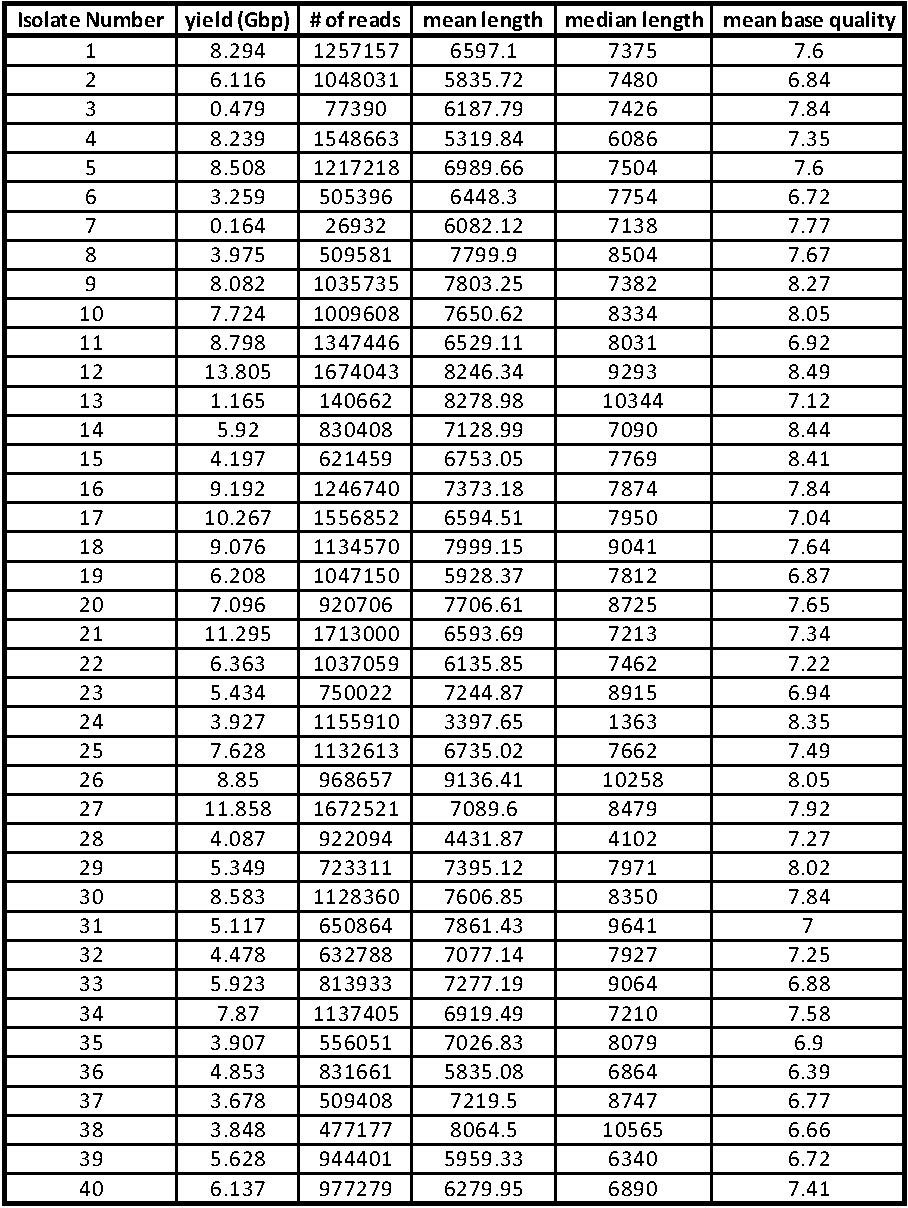
\includegraphics[width = .7\linewidth,keepaspectratio]{figure/runnanopore.pdf}
\caption[Nanopore sequencing data]{{\bf Nanopore sequencing data.} Summary of nanopore sequencing data for each isolate }
\label{tab:runnanopore}
\end{table}


\begin{table}[!ht]
\centering
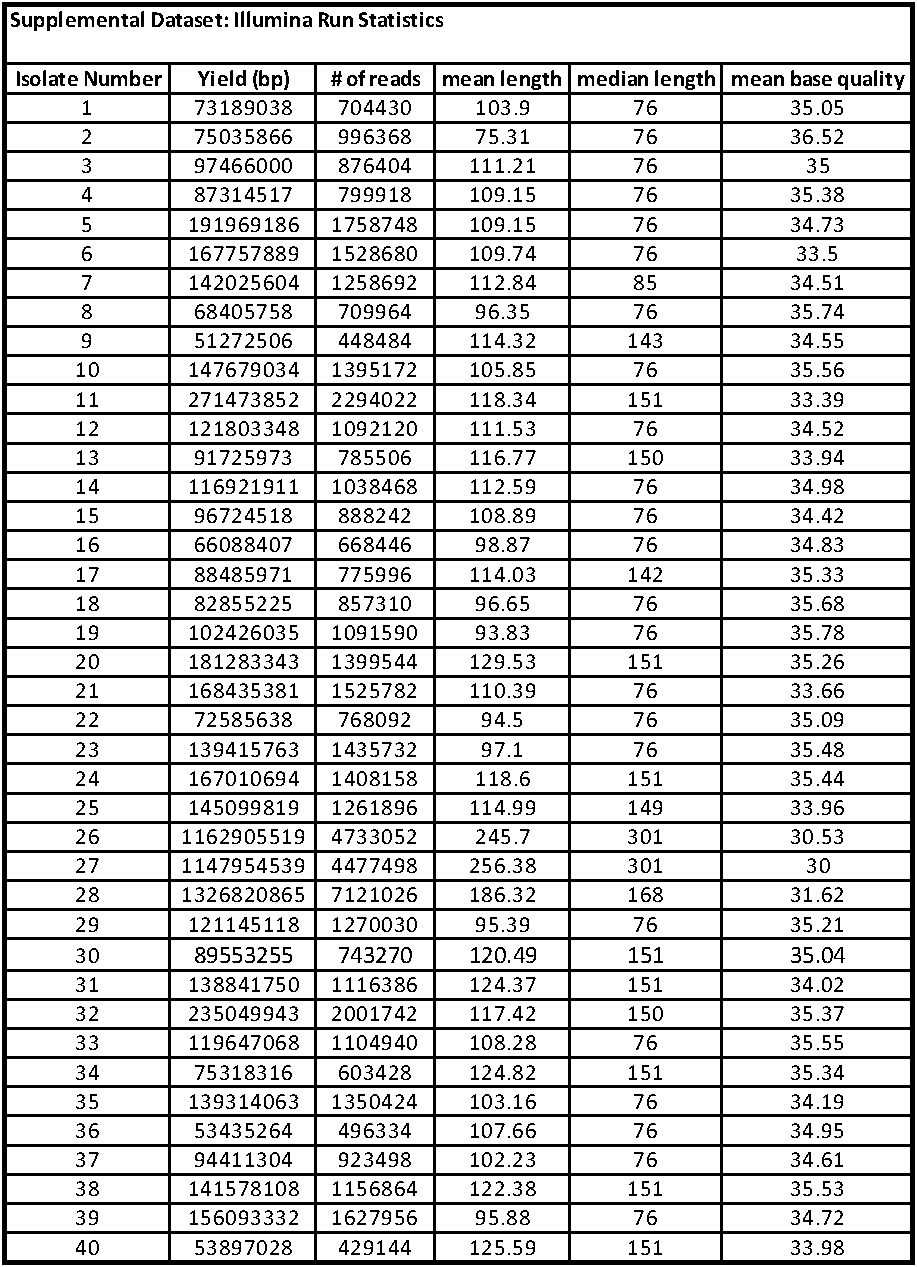
\includegraphics[width = .7\linewidth,keepaspectratio]{figure/runillumina.pdf}
\caption[Illumina sequencing data]{{\bf Illumina sequencing data.} Summary of Illumina sequencing data for each isolate }
\label{tab:runillumina}
\end{table}


\begin{figure}[!ht]
\centering
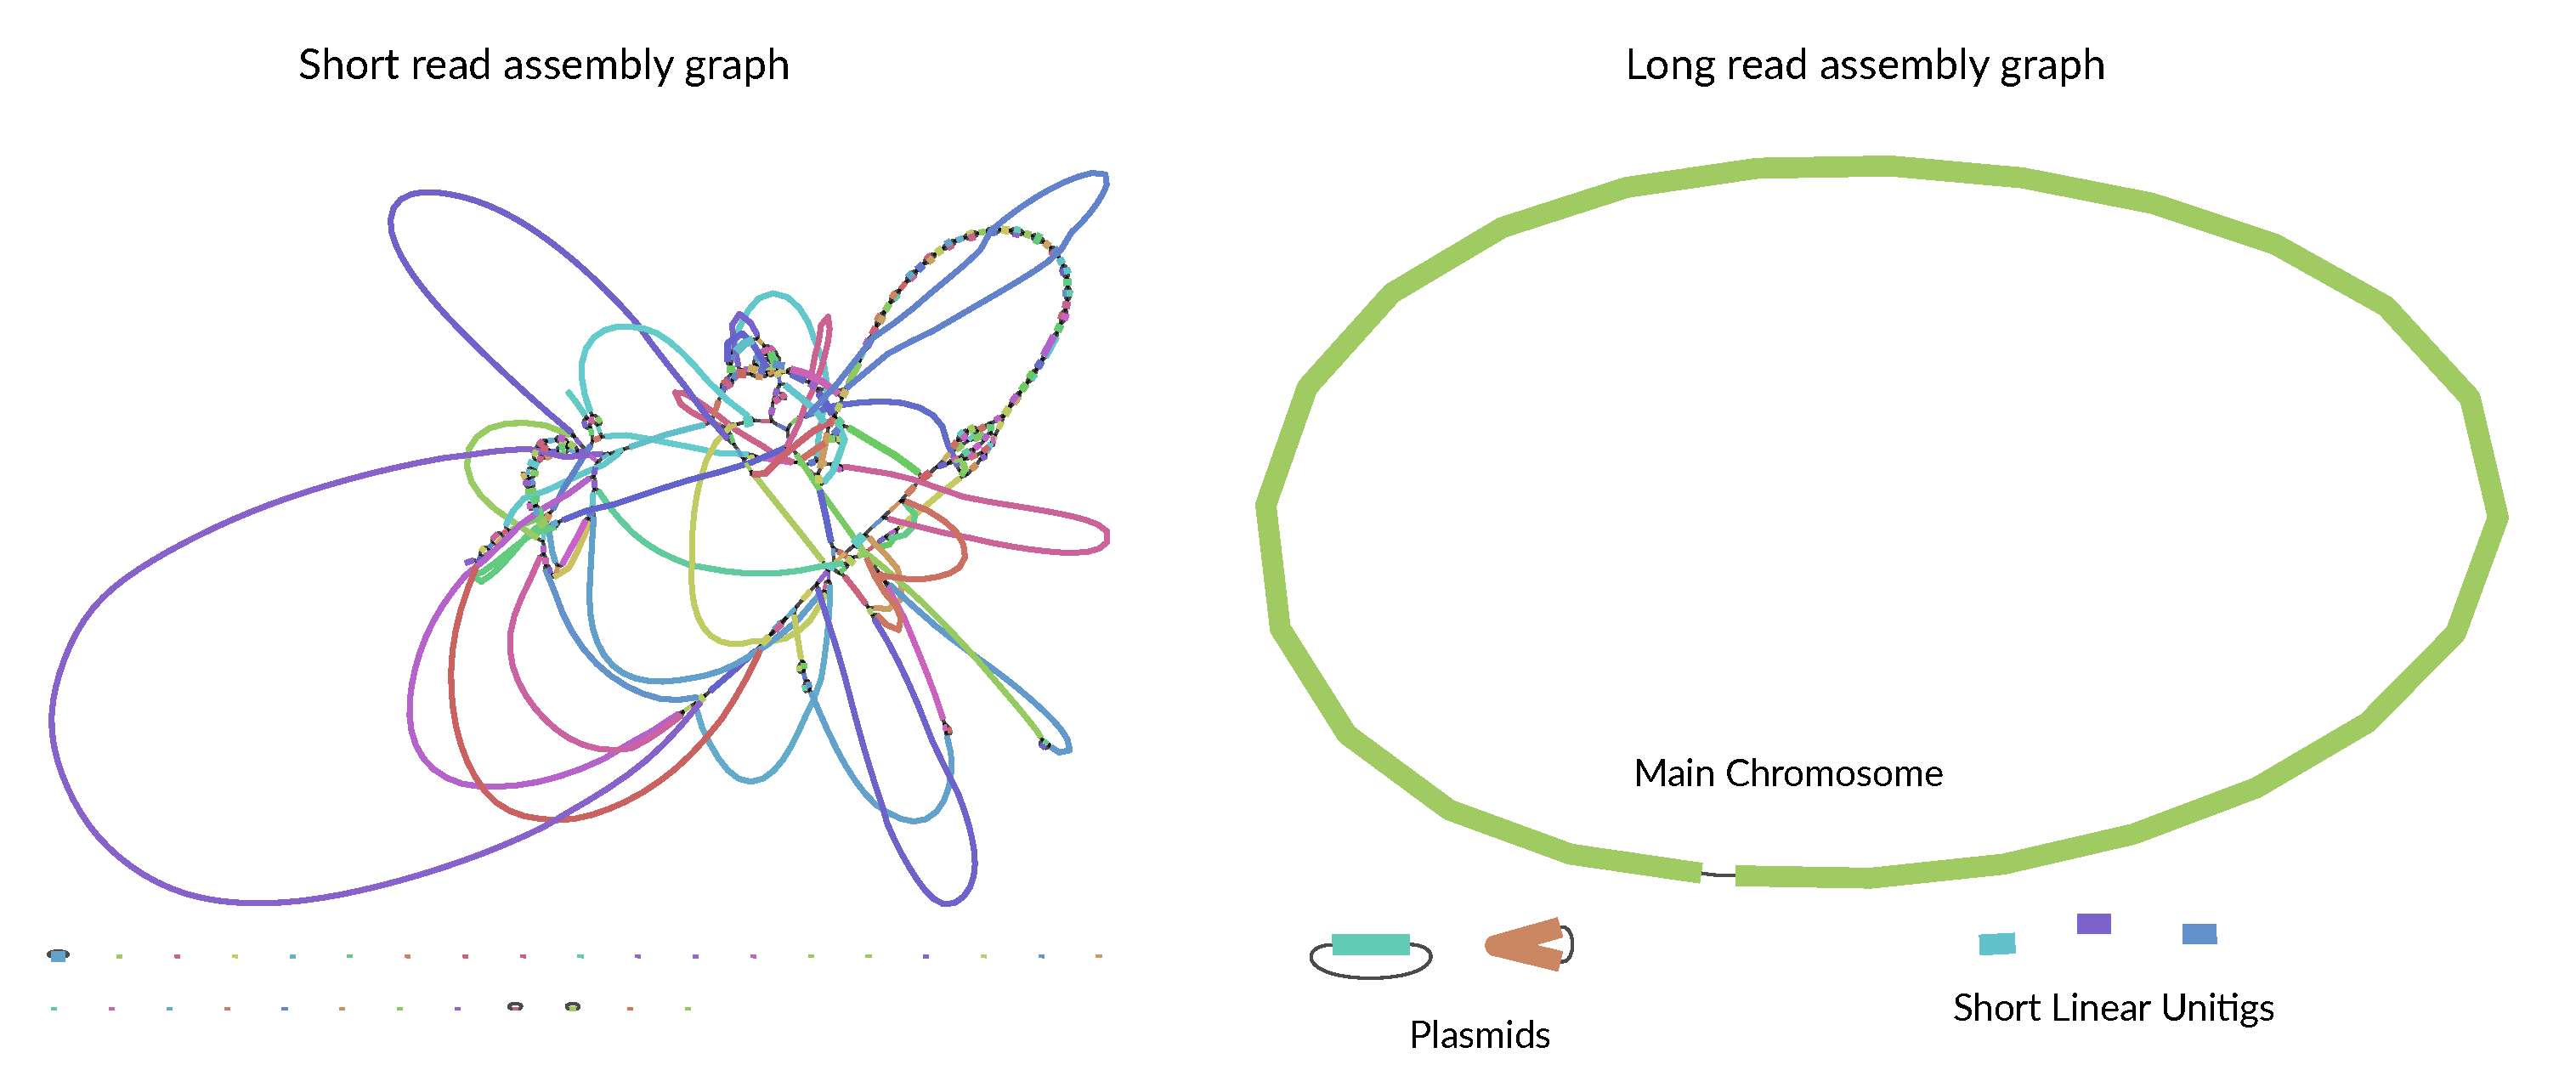
\includegraphics[width = 1\linewidth,keepaspectratio]{figure/graphsasm.pdf}
\caption[Assembly graphs]{{\bf Assembly graphs.} Representative assembly graphs when using only short reads and only long reads. Short reads are difficult to use for resolving repetitive regions, resulting in bubbles in the graph, whereas assemblies from long read data typically result in a full length bacterial chromosome. }
\label{fig:graphsasm}
\end{figure}


\begin{table}[!ht]
\centering
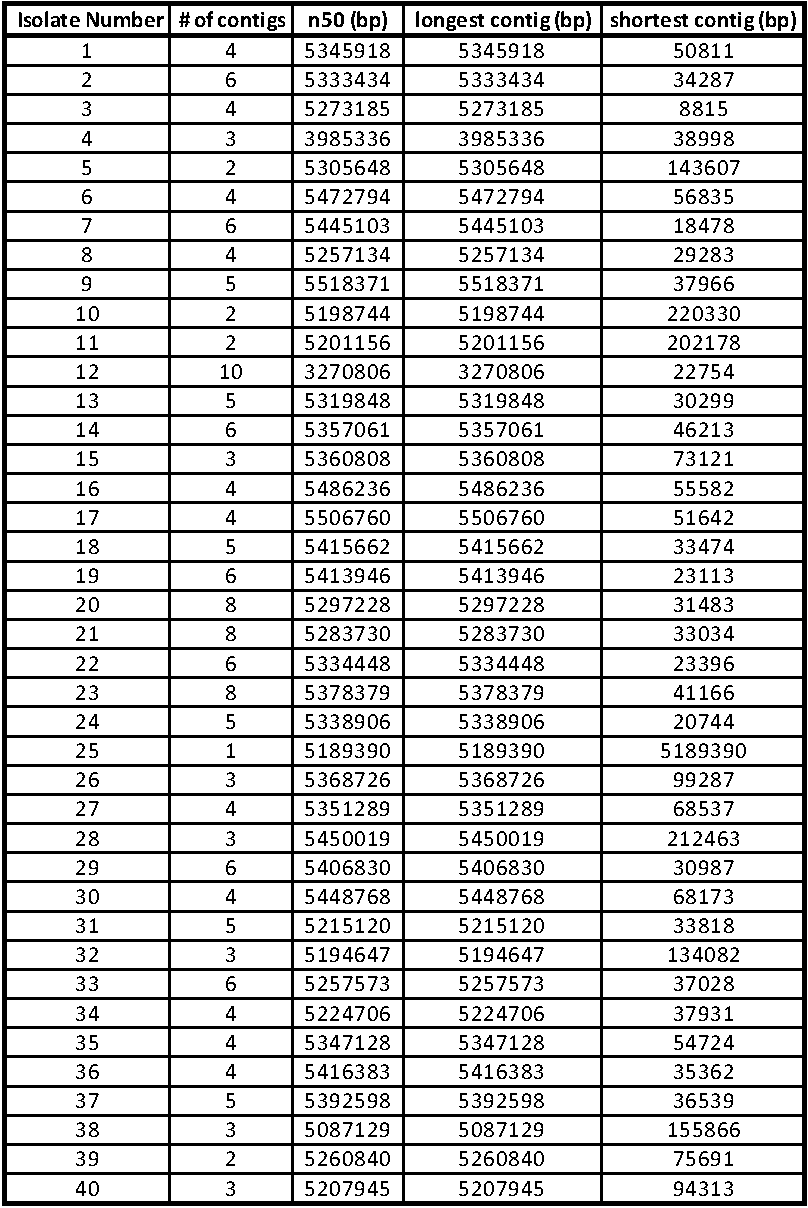
\includegraphics[width = .7\linewidth,keepaspectratio]{figure/asmraw.pdf}
\caption[Raw assembly statistics]{{\bf Raw assembly statistics.} Summary statistics for genome assemblies of all isolates with no further correction }
\label{tab:asmraw}
\end{table}


\begin{table}[!ht]
\centering
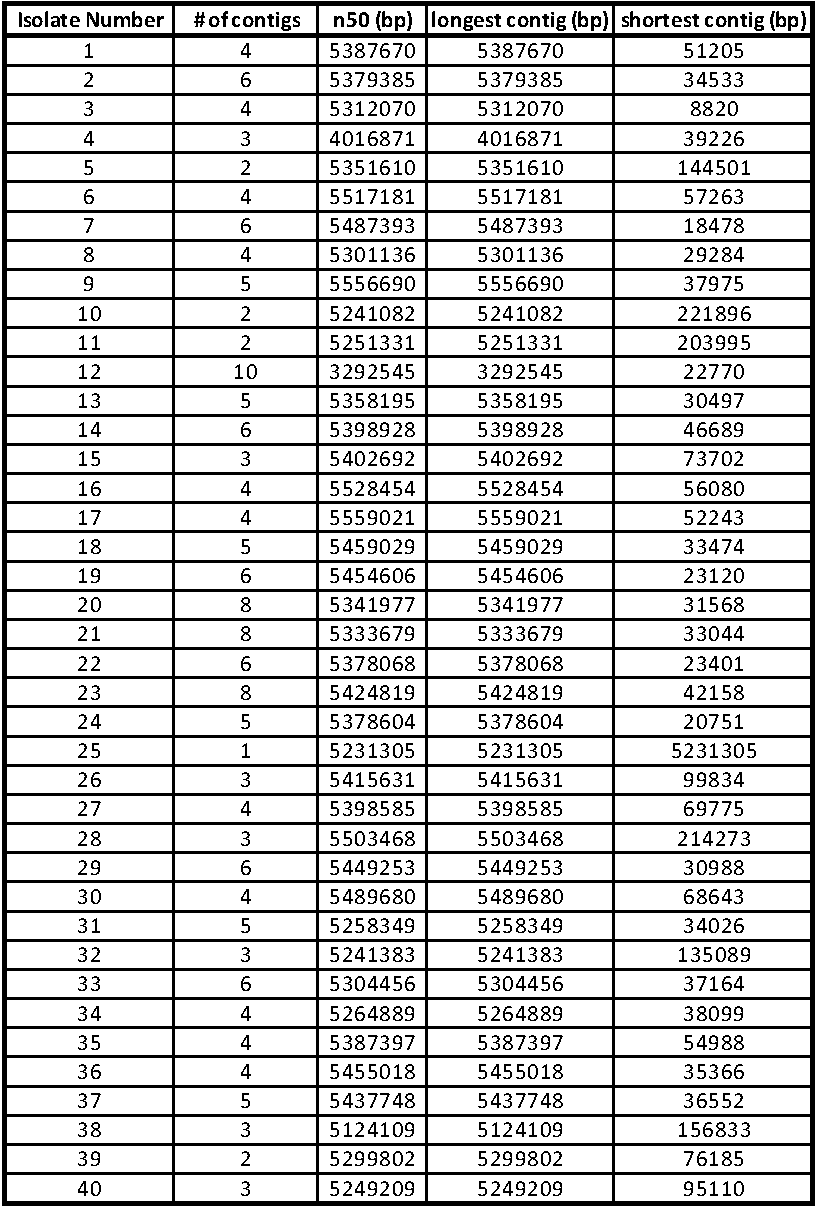
\includegraphics[width = .7\linewidth,keepaspectratio]{figure/asmpolished.pdf}
\caption[Polished assembly statistics]{{\bf Polished assembly statistics.} Summary statistics for genome assemblies of all isolates after correction with nanopolish }
\label{tab:asmpolished}
\end{table}


\begin{table}[!ht]
\centering
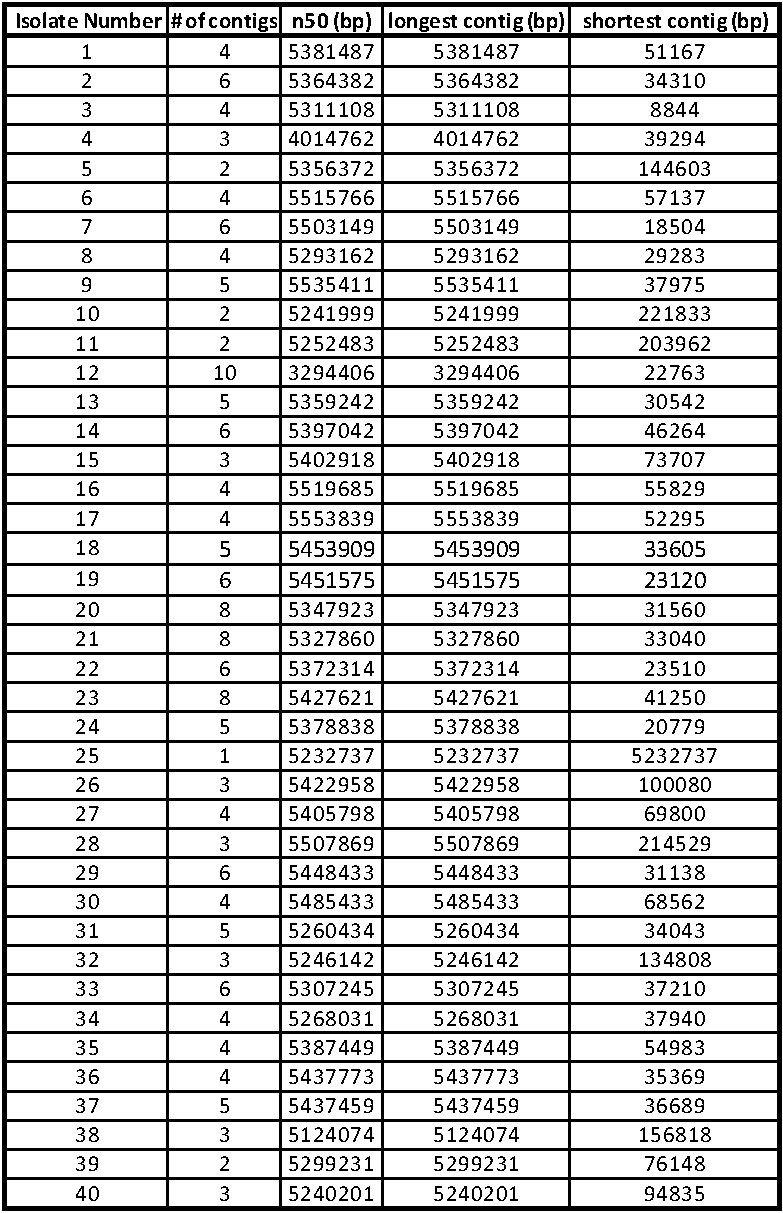
\includegraphics[width = .7\linewidth,keepaspectratio]{figure/asmpilon.pdf}
\caption[Short-read correction assembly statistics]{{\bf Short-read correction assembly statistics.} Summary statistics for genome assemblies of all isolates after correction with short-read data }
\label{tab:asmpilon}
\end{table}


\begin{table}[!ht]
\centering
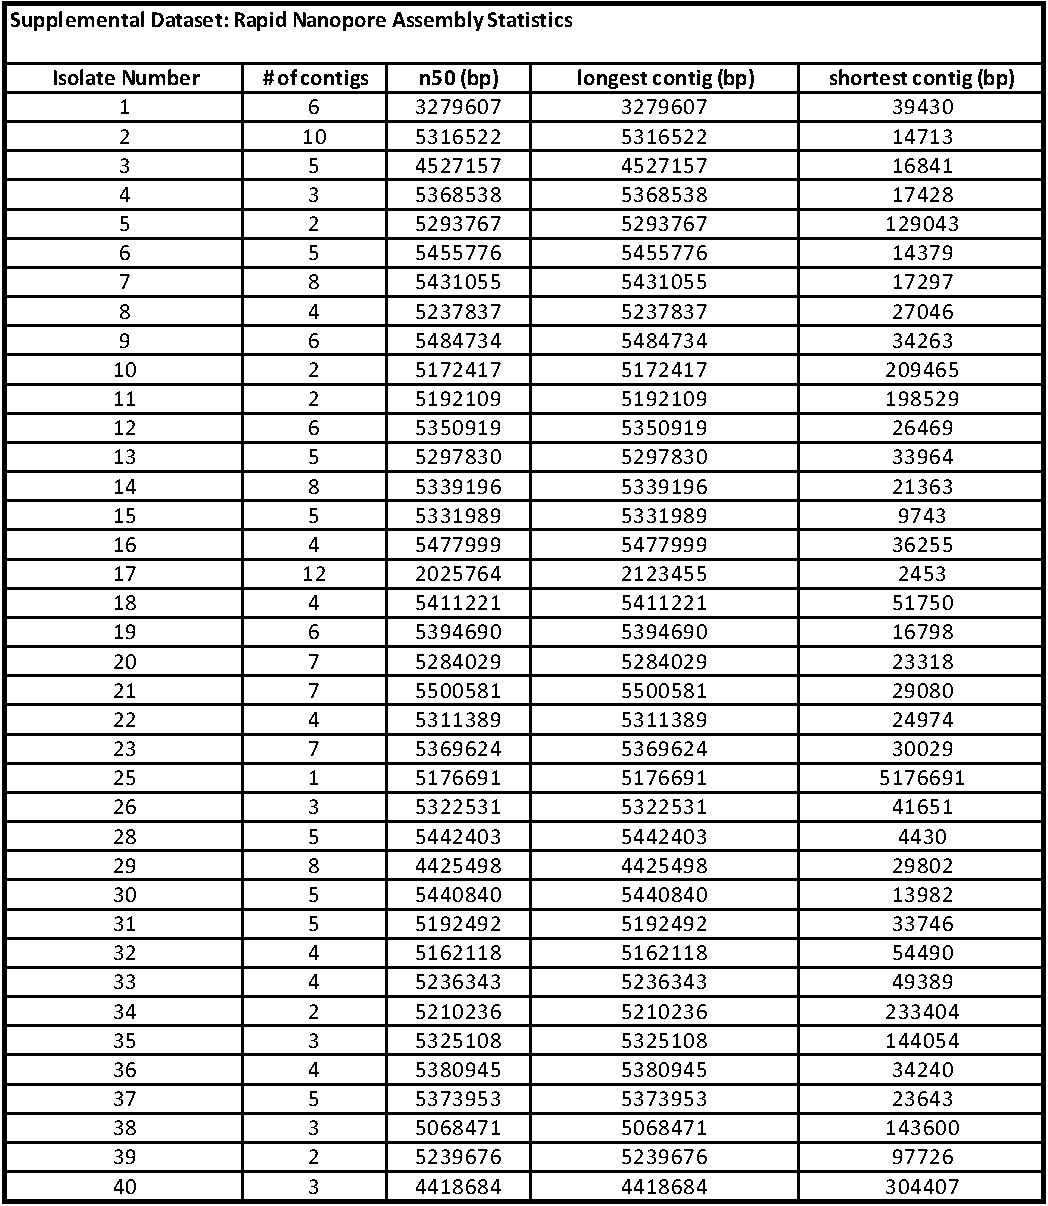
\includegraphics[width = .7\linewidth,keepaspectratio]{figure/asmrapid.pdf}
\caption[Rapid assembly statistics]{{\bf Rapid assembly statistics.} Summary statistics for genome assemblies of all isolates using downsampled data }
\label{tab:asmrapid}
\end{table}


\begin{figure}[!ht]
\centering
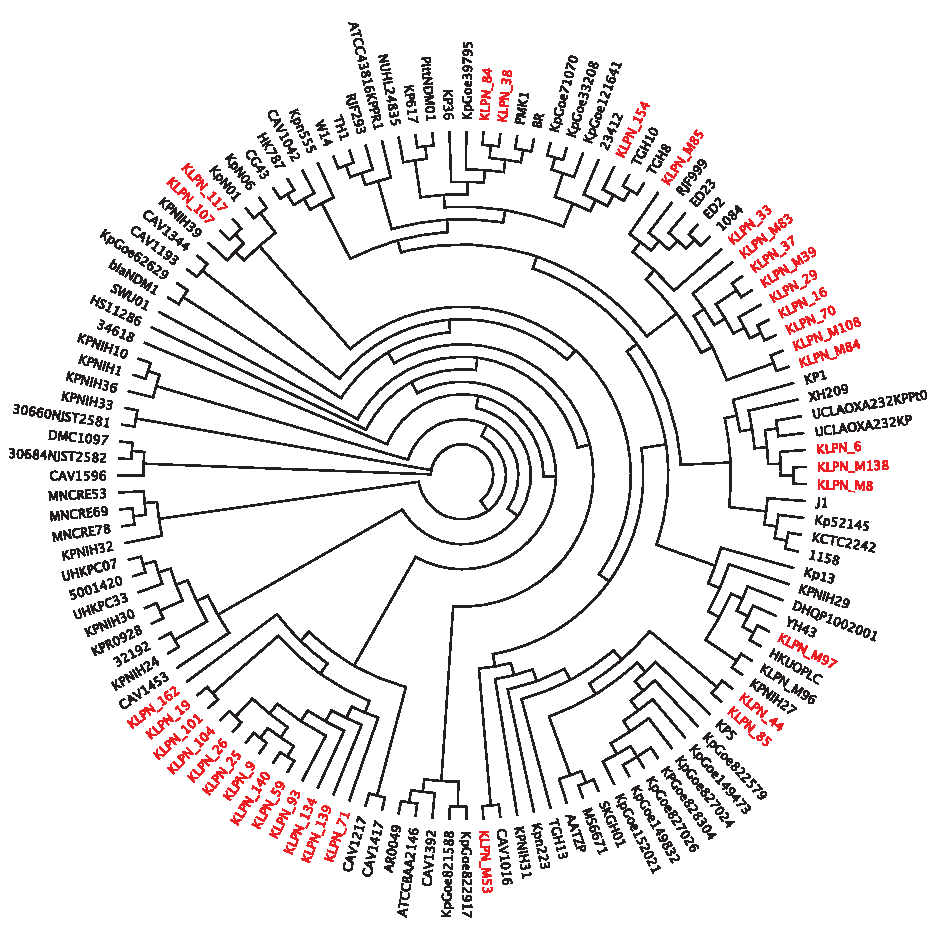
\includegraphics[width = .9\linewidth,keepaspectratio]{figure/tree.pdf}
\caption[Phylogenetic tree of \textit{K. pneumoniae} genomes]{{\bf Phylogenetic tree of \textit{K. pneumoniae} genomes.} Isolates from this study are shown in red, and chromosome-level genomes obtained from GenBank are shown in black. }
\label{fig:tree}
\end{figure}


\subsection{Percent agreement of WGS in predicting AST results}
\label{sec:agree}

The overall agreement of genotypic results and anticipated AST results for the 40 \textit{K. pneumoniae} isolates was 77\% (range, 30\% to 100\%), 92\% (range, 80\% to 100\%), and 92\% (range, 80\% to 100\%) for the Nanopore real-time approach, the Nanopore sequencing assembly approach, and the Pilon-corrected Illumina approach, respectively ({\bf Table \ref{tab:astagreement}}). The Nanopore real-time approach, compared to the assembly-based approach, had an inability to identify allelic variants (i.e., \textit{bla}\textsubscript{KPC} was identified but \textit{bla}\textsubscript{KPC-3} could not be specifically identified). Because all \texit{K. pneumoniae} isolates are known to have chromosomally integrated non-ESBL {\textbeta}-lactamase genes (e.g., \textit{bla}\textsubscript{SHV-1}, \textit{bla}\textsubscript{SHV-11}), when \textit{bla}\textsubscript{SHV} was identified, the assumption was that it was a non-ESBL \textit{bla}\textsubscript{SHV}. This led to reductions in the accuracy of predictions for several {\textbeta}-lactams, including 5\%, 2\%, and 3\% reductions in accurate predictions for piperacillin-tazobactam, ceftriaxone, and cefepime, respectively. Also, since the number of aminoglycoside-modifying enzymes were important to predict aminoglycoside resistance, and the alleles could not be distinguished, this led to decreases in accurate predictions for amikacin (reduced by 7\%) and gentamicin (reduced by 48\%). Additionally, the real-time approach was unable to identify chromosomal mutations, leading to decreases in accurate predictions for ciprofloxacin/levofloxacin (reduced by 68\%) and colistin (reduced by 5\%).

\begin{table}[!ht]
\centering
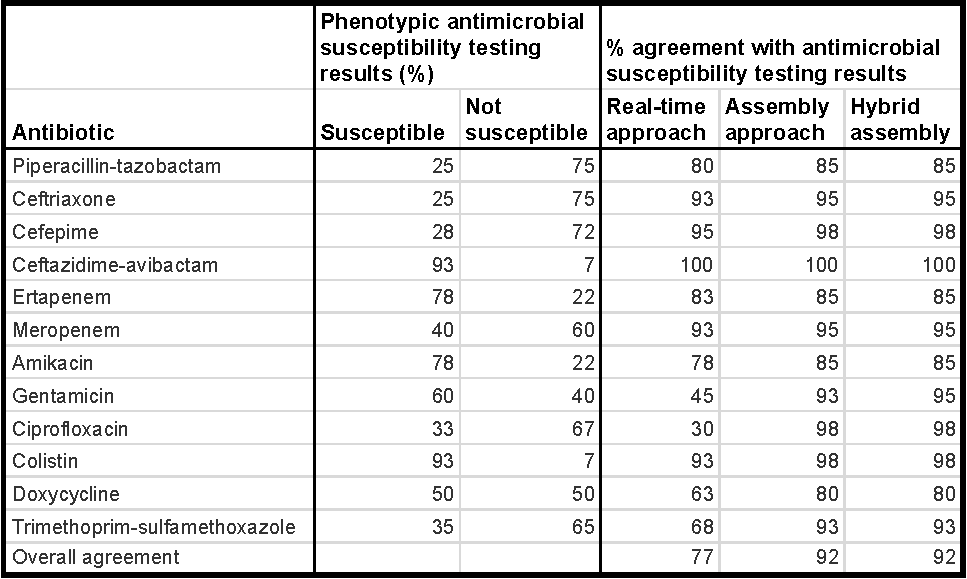
\includegraphics[width = 1\linewidth,keepaspectratio]{figure/astagreement.pdf}
\caption[WGS vs phenotypic AST]{{\bf WGS vs phenotypic AST.} Percent agreement between three different sequencing and analysis approaches compared to phenotypic antimicrobial susceptibility testing results for 40 \textit{Klebsiella pneumoniae} clinical isolates }
\label{tab:astagreement}
\end{table}


\subsection{Time to resistance determination}
\label{sec:time}

With a Nanopore real-time analysis approach, acquired resistance genes were identified within 8 h from subcultured isolates. Assemblies sufficient for full resistance gene and single-nucleotide polymorphism annotation using Nanopore sequences (Nanopore assembly approach) were available within 14 h from subcultured isolates. {\bf Figure \ref{fig:timeline}} compares the Nanopore real-time analysis and assembly approaches with standard-of-care methods. {\bf Table \ref{tab:astagreement}} summarizes the agreements between antibiotic resistance determinants identified using the real-time approach, assembly-based approach, or hybrid Nanopore-Illumina assemblies and AST predictions.

\begin{figure}[!ht]
\centering
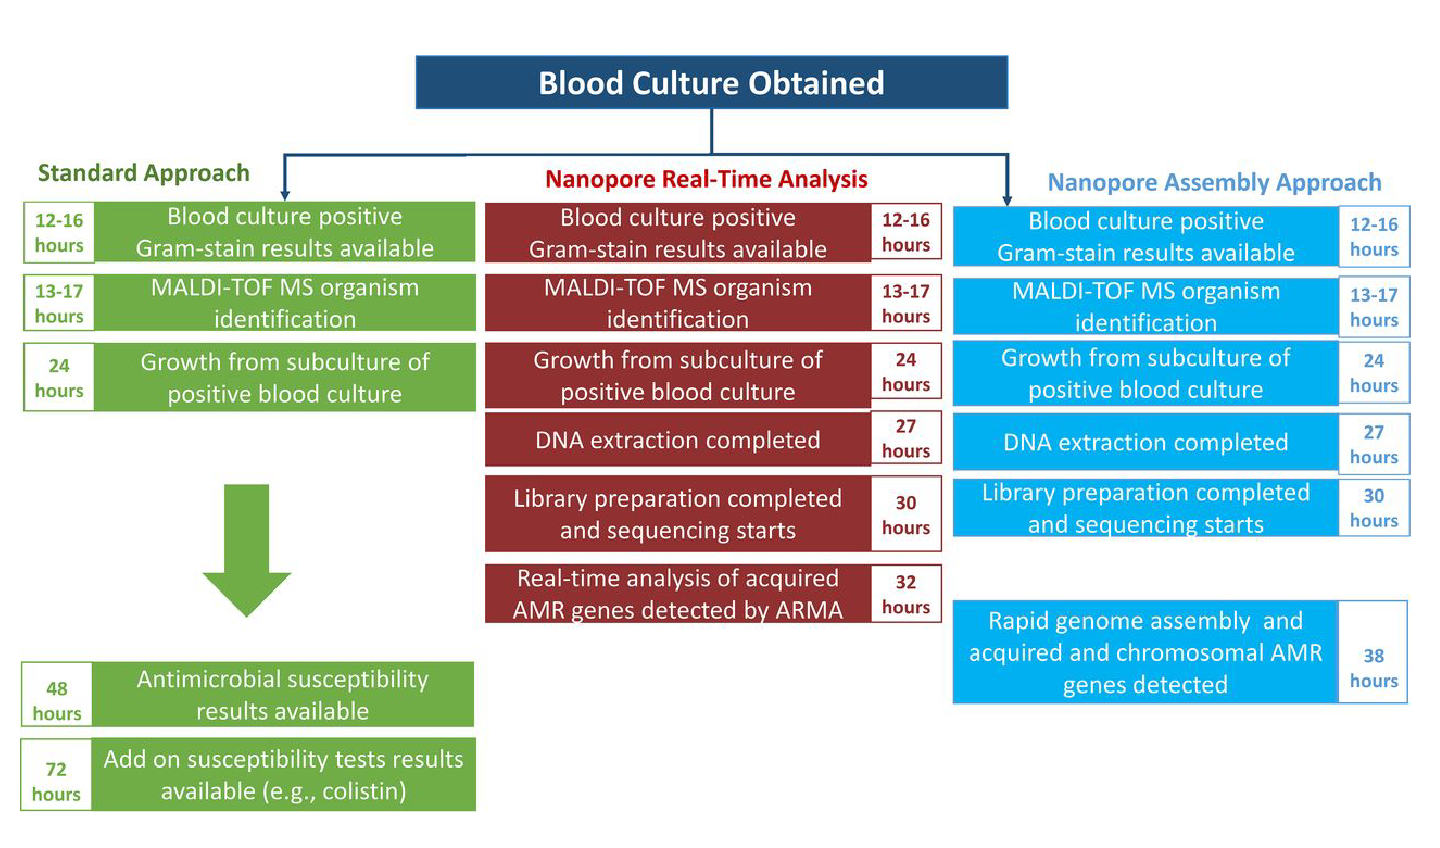
\includegraphics[width = 1\linewidth,keepaspectratio]{figure/timeline.pdf}
\caption[Estimated timelines of resistance detection]{{\bf Estimated timelines of resistance detection.} Schematic of Nanopore sequencing with a real-time analysis and assembly-based approach for identifying resistance genes compared to standard of care testing, using an example of a positive blood culture. MALDI-TOF MS, matrix-assisted laser desorption ionization<U+2013>time of flight mass spectrometry; AMR, antimicrobial resistance; AST, antimicrobial susceptibility testing. }
\label{fig:timeline}
\end{figure}


There were 28 patients in the cohort infected with carbapenem-resistant \textit{K. pneumoniae} strains. Overall, 22 (79\%) received empirical antibiotic therapy that was not active against their infecting isolates. Results from Nanopore sequencing with assembly approach had the potential to place 20 (91\%) of these patients on effective therapy sooner than did standard AST methods.

Overall, the median time to effective antibiotic therapy for the 28 patients infected with carbapenem-resistant \textit{K. pneumoniae} was 61 h (interquartile range [IQR], 43 to 82 h). Of the antibiotics evaluated, ceftazidime-avibactam, extended-infusion meropenem, aminoglycosides, fluoroquinolones, polymixins, and tigecycline are generally considered reasonable treatment options for infections caused by carbapenem-resistant \textit{K. pneumoniae} isolates, if active in vitro. As results from the real-time analysis approach were generally available within 8 h from subcultured isolates, Nanopore real-time analysis could have led to an average time to effective therapy of 41 h (IQR, 33 to 44). Using the Nanopore assembly approach, time to effective therapy could have been reduced to 35 h (IQR, 32 to 42). The time to effective therapy was reduced with the assembly approach compared to that with the real-time approach because the former provided more comprehensive data to infer AST activity (e.g., aminoglycoside resistance, colistin resistance, etc.) than the real-time approach, for which there were delays in antibiotic optimization while awaiting additional AST results. Both the real-time and assembly approaches were significantly faster than the standard approach.


\section{Discussion}
\label{sec:discuss}

Our results demonstrate that Nanopore sequencing can be employed to both accurately and rapidly predict phenotypic AST profiles. Our study builds off previously published proof-of-concept or early insight studies applying Nanopore sequencing for the detection of antimicrobial resistance genes \citep{Judge2015-zw, Judge2016-ds, Li2019-op, Van_der_Helm2017-ww, Xia2017-ss, Neuert2018-il, Hasman2014-el, Stoesser2013-se}. We found an overall agreement of 92\% between genotypic results and comprehensive AST results using a Nanopore assembly-based approach. We further demonstrated that assembly-based approaches enhance the ability to identify chromosomal mutations and allelic variants compared to that of the Nanopore real-time approach. A future method centered on real-time alignment and consensus of raw reads to a database of antimicrobial resistance (AMR) genes will enhance the capabilities of the real-time approach. Nevertheless, even with its current limitations, the Nanopore real-time analysis approach correctly predicted the presumed activity of a number of antibiotics commonly prescribed for Gram-negative infections, such as {\textbeta}-lactams, trimethoprim-sulfamethoxazole, tetracyclines, with reasonable accuracy, with full annotation of acquired AMR genes within 8 h from the time of cultured isolates. Within 14 h of cultured isolates, a Nanopolished assembly-based approach would allow for predictions of the activity of additional agents, such as fluoroquinolones, aminoglycosides, and polymixins (beyond \textit{mcr}-1 and its variants), due to the ability to detect chromosomal mutations or allelic variants leading to resistance. We believe that with rapid extraction and library preparation techniques, the turn-around times could further be reduced to 	{\textless}3 h for a real-time approach and {\textless}9 h for a Nanopore assembly-based approach. Moreover, using a hypothetical trial design, we found that a real-time approach and assembly approach could shorten the average time to effective antibiotic therapy for carbapenem-resistant \textit{K. pneumoniae} infections by 20 h and 26 h, respectively, compared to standard approaches.

Although there have been other investigations of the use of WGS to predict AST results for Gram-negative organisms based on resistance determinants \citep{Shelburne2017-dm, Cao2016-oj, Schmidt2017-ng, Lemon2017-td, Judge2015-zw, Judge2016-ds, Li2019-op, Van_der_Helm2017-ww, Xia2017-ss, Stoesser2013-se}, ours is the first to use a Nanopore assembly approach for evaluating a broad range of acquired resistance genes and chromosomal mutations in predicting susceptibility results for a comprehensive panel of antibiotics. Previous studies applying Nanopore sequencing for resistance gene detection have applied this methodology to small numbers of isolates and limited evaluations to acquired resistance genes. Furthermore, the potential impact of WGS in reducing time to appropriate antibiotic therapy for highly drug-resistant organisms has not been previously reported. As the science of WGS continues to evolve, the costs of sequencing are becoming more affordable, and the time requirements for DNA extraction, library preparation, assembly, and detection are anticipated to be further reduced. We believe that this methodology can accurately expedite antibiotic decision making for critically ill patients infected with MDRGN organisms. WGS also provides the ability to identify emerging mechanisms of resistance, such as \textit{mcr} variants or novel mechanisms of resistance against newly approved agents \citep{Haidar2017-pk, Haidar2017-rw}.

As we continue to gain further insights into the complexities of resistance mechanisms present in Gram-negative organisms, it is becoming increasingly clear that sole reliance on the detection of {\textbeta}-lactamase genes to identify antibiotic resistance is insufficient. Such is the case with commercially available PCR-based methodologies (e.g., Cepheid Xpert Carba-R assay, BioFire FilmArray blood culture identification panel, Verigene Gram-negative blood culture test, etc.) that fail to identify the wide array of additional resistance determinants (e.g., porin deletions, multidrug efflux pumps, functioning of the two-component regulatory system, DNA gyrase mutations, off-panel targets, etc.). Using carbapenem-resistant \textit{K. pneumoniae} as a case study, over half of isolates render carbapenem antibiotics ineffective due to non-carbapenemase-mediated mechanisms \citep{Tamma2017-el}. Similarly, carbapenem resistance among Pseudomonas aeruginosa strains in the United States is predominantly mediated by noncarbapenemase mechanisms, including the loss of OprD porin expression and/or upregulation of MexAB-OprM efflux pumps \citep{Lister2009-ex}. WGS offers a more comprehensive approach to identifying clinically relevant antibiotic resistance compared with standard PCR technologies.

Nanopore technology offers real-time DNA sequencing of long reads, which facilitate the process of high-quality genome assembly \citep{Lu2016-ru}. Additionally, they are better able to capture large regions of structural variation (e.g., insertions, deletions, duplications, translocations, inversions, etc.) and resolve repetitive regions accurately, compared to technologies which generate short-read data. However, there are some drawbacks to Nanopore sequencing \citep{Lu2016-ru}. Chromosomal mutations as small as single-base polymorphisms in DNA can result in drastic changes to proteins due to frame shifts or early truncations. Indels and resulting false positives in chromosomal mutations can be difficult to distinguish with Nanopore sequencing alone \citep{Jain2018-qp}. The assembly process generally removes random error, given sufficient sequencing coverage. However, systematic errors in the form of homopolymer indels and methylation errors still result in disagreement compared with Illumina-corrected assemblies. Nanopolish corrects most homopolymer indels, improving accuracy, but in its current form, it is not all-inclusive \citep{Loman2015-nf}. Methylation motifs alter the electrical signal from Nanopore sequencing, resulting in errors in base calling. We anticipate further improvements to the quality of Nanopore sequencing and available bioinformatics, enabling this technology to rapidly and accurately resolve variants of acquired resistance genes and characterize chromosomal mutations in the absence of assembly.

We assessed the minimum sequencing time to be able to accurately predict AST using Nanopore sequencing. We determined that a minimum of 10 reads per gene were required and that a sequencing run of 1 h is sufficient to predict the AST profile, using either a real-time ARMA or an assembly approach. In fact, we were able to detect 10 reads of all AMR genes within 14 min of starting the sequencing run and 40 reads of each gene within 1 h. This is an important quality control measure as we begin to consider these methods for clinical application.

There are several remaining limitations to this work. First, there were some antimicrobial susceptibility profiles for which we were unable to identify the associated resistance mechanisms, suggesting that our approach to resistance detection was not comprehensive. As an example, we were only able to accurately predict piperacillin-tazobactam activity 85\% of the time. This is similar to what others have shown \citep{Shelburne2017-dm}, and it is likely due to efflux pumps, where expression analysis is required. Second, there were some agents tested for which no resistance was observed (e.g., tigecycline), precluding us from including these agents in our analysis. Third, we only evaluated \textit{K. pneumoniae} isolates from a single region of the United States. Validation needs to occur in larger data sets with a more diverse array of genera and species and resistance mechanisms, including some not observed in our isolates, such as the \textit{mcr} genes. Additionally, as antibiotic susceptibility criteria include several considerations, such as wild-type MIC distributions, pharmacokinetic-pharmacodynamic modeling, clinical outcomes data, etc., it can be challenging to determine the most accurate MIC that signifies nonsusceptibility. The European Committee on Antimicrobial Susceptibility Testing suggests that epidemiologic cutoff values (i.e., wild-type versus non-wild-type distributions) are the preferred values for correlation with resistance genes \citep{Eucast_undated-wa}. We elected to use antibiotic breakpoints, as these remain the most relevant metric for quantifying antibiotic resistance for clinicians, but we realize that this might not be the most accurate proxy.

In conclusion, we were able to leverage the long reads, rapid turnaround time, and real-time analytic capabilities of Nanopore sequencing to accurately identify resistance loci. With the continued rise in highly drug-resistant infections, the need for rapid and accurate methods to detect antibiotic resistance is becoming increasingly important. Continued enhancements to WGS may permit real-time AMR gene detection from clinical isolates in the near future.

\section{Materials and Methods}
\label{sec:methods}

\subsection{Study cohort}
\label{sec:cohort}

Forty clinical \textit{Klebsiella pneumoniae} complex isolates collected between 2016 and 2017 and processed at the Johns Hopkins Hospital Medical Microbiology Laboratory were included in the present study. Isolates for inclusion were deliberately selected based on their diversity of AST results and mechanisms of resistance and included 30 carbapenem-resistant (21 carbapenemase producers and 10 non-carbapenemase producers) and 9 carbapenem-susceptible \textit{K. pneumoniae} isolates. As this was a proof-of-concept study comparing different WGS approaches, we decided to focus on a single genus and species (i.e., \textit{K. pneumoniae}) to increase the number of isolates with any single resistance mechanism identified, as some resistance mechanisms are genus and species specific, especially among chromosomal mutations leading to resistance. Isolates were subcultured from frozen stock to tryptic soy agar (TSA) with 5\% blood agar. A second subculture was performed prior to DNA extraction. \textit{K. pneumoniae} isolates from deep tissue (n = 3), intraabdominal fluid (n = 1), blood (n = 10), respiratory (n = 10), and urine (n = 16) were included.

\subsection{Species and antimicrobial susceptibility testing}
\label{sec:ast}

Bacterial genus and species were identified using matrix-assisted laser desorption ionization–time of flight mass spectrometry (Bruker Daltonics Inc., Billerica, MA). AST results were determined using the BD Phoenix Automated System NMIC-303 panels (BD Diagnostics, Sparks, Maryland). MICs were confirmed by broth microdilution (BMD) with Sensititre GNX2F Gram-negative panels (Thermo Fisher Scientific, Indianapolis, IN) and the ceftazidime-avibactam Etest (bioMérieux, France) \citep{Matuschek2018-qh}. BMD was repeated on isolates with 2-fold or greater MIC discrepancies between the Phoenix automated panel and initial BMD results. Interpretive criteria established by the Clinical and Laboratory Standards Institute (CLSI) were used to define antibiotic susceptibility. AST results in both the “intermediate” and “resistant” ranges were categorized as resistant.

\subsection{Whole-genome sequencing and antimicrobial resistance gene detection}
\label{sec:wgs}

As Nanopore sequencing has a substantial raw sequencing error rate, three separate sequencing and analysis pipelines were performed, as follows: (i) a real-time Nanopore (Oxford, England) analysis approach that identified acquired and chromosomal resistance genes by applying Metrichor’s Antimicrobial Resistance Mapping Application (ARMA) (https://nanoporetech.com/resource-centre/real-time-detection-antibiotic-resistance-genes-using-oxford-nanopore-technologies); (ii) an assembly-based Nanopore approach that uses Canu and Nanopolish \citep{Loman2015-nf, Koren2017-wf} to compute high-identity sequences with identification of resistance genes, using Abricate ResFinder results as well as chromosomal mutations (e.g., ompK35 and ompK36 mutations, \textit{gyrA} and \textit{parC} mutations, etc.) from genomic assemblies, using minimap2 \citep{Li2018-eq} and a tool evaluating the impact on amino acid translation based on resulting codon changes (https://github.com/gpertea/pwasm); and (iii) a Pilon-corrected hybrid approach using both Illumina (Illumina, San Diego, California) and Nanopore sequencing \citep{Walker2014-eh}. The short-read correction of Nanopore assemblies served as the reference standard to determine the accuracy of Nanopore sequencing results.

Long-read genomic sequencing was performed using the third generation Oxford Nanopore MinION MkIb (Isolates 1-30) and GridION X5 (Isolates 31-40; Oxford, England) sequencing instruments. Genomic DNA was extracted from pure cultures using the DNeasy PowerBiofilm Kit (Qiagen, Hilden, Germany). Each Nanopore sequencing library was prepared using 5 µg of DNA with the 1D ligation kit (SQK-LSK108, Oxford Nanopore Technologies) using R9.4 flowcells (FLO-MIN106). A single isolate was run per flowcell. MinKNOW software was used to collect sequencing data.

For the real-time analysis approach, the Oxford Nanopore Technology “What’s In My Pot” (WIMP) \citep{Juul2015-zt} and Metrichor’s Antimicrobial Resistance Mapping Application (ARMA) real-time analysis tools were run in parallel to both sequencing and base-calling. WIMP uses a customized pipeline applying the Centrifuge metagenomic classifier to the sequencing reads. ARMA aligns sequencing reads to the Comprehensive Antimicrobial
Database (CARD) \citep{Jia2017-pg}, identifying antimicrobial resistance (AMR) gene hits.

For the assembly-based approach, Albacore v2.1.3 was used to base-call. Raw data were corrected, trimmed, and assembled using Canu v1.6 \citep{Koren2017-wf} using default parameters. Genome size was assumed to be 5.3Mb. For isolates that did not assemble under default parameters, either read quality restrictions were relaxed or minimum overlap requirements were shortened as suggested by the software documentation. Assembled contigs were screened for resistance genes using Abricate (https://github.com/tseemann/abricate), a tool that uses alignment to search for resistance gene sequences from several database including ResFinder, CARD, ARG-ANNOT, and the NCMI AMR Reference Gene Database. ResFinder results were evaluated in this study \citep{Zankari2012-uk}. In a separate experiment, we were able to build high quality genomes from nanopore electrical data in under 6 hours using a machine with 36 cores and 72GB RAM. Thirteen random blocks of 4000 reads were sampled and taken through basecalling, assembly and polishing. Conservatively, it takes at most an hour to reach 52,000 reads on a typical run.

WGS was also conducted using Illumina MiSeq short-read sequencing to increase assembly accuracy (Illumina, San Diego, California). A drawback with Illumina sequencing is the turn-around time as sequencing alone requires between 19-24 hours for 300 cycles. As the ultimate goal would be to use Nanopore sequencing alone for both resistance gene and chromosomal mutation identification, in the current analysis, the Pilon-corrected assemblies were not meant to supplant or supplement Nanopore sequencing but rather to serve as a reference standard to determine the accuracy of Nanopore sequencing results. Approximately 100-500 ng of gDNA was used to prepare sequencing libraries using the Nextera Flex Kit. The each Illumina library was then sequenced using both v2 2x150 and v3 2x75 reagents on an Illumina Miseq. These reads were used to correct the more error prone Nanopore assembly with the Pilon v1.22 software package in conjunction with the short-read aligner Bowtie2 v2.2.6. Phylogenetic trees were generated using Parsnp v1.2 \citep{Treangen2014-bu}.

\subsection{Predicted correlations between WGS and AST results}
\label{sec:wgsast}

Predictions of resistance were performed without reference to phenotypic data, unless otherwise noted in Results. The correlations of resistance genes and sequence variants with anticipated AST results for the evaluated antibiotics were determined based on reference gene databases and the published literature \citep{Bush2010-lg, Bush1995-rb, Jacoby2009-wr, Naas2008-vx, Evans2014-md, Zhang2014-xg, Feng-Jui2003-nf, Vetting2011-iu, Kim2009-me, Ramirez2010-sv, Galimand2012-gu, Liakopoulos2016-wl, Tarnberg2009-qg, Bonnet2004-xz, Roberts2005-js, Fevre2005-vm, Fu2013-cm, Poirel2010-ch}. Antimicrobial resistance genes and mutation results were reviewed manually to predict AST results. For associations for which ambiguity existed, the following rules were established a priori:
\begin{itemize}
  \item SHV 2be extended-spectrum {\textbeta}-lactamase enzymes were assumed to inactivate ceftriaxone and cefepime if they contained G238S or E240K mutations \citep{Liakopoulos2016-wl, Howard_Christopher2002-tr}
  \item The relative contributions of porins OmpK35 and/or OmpK36 truncations to {\textbeta}-lactam resistance have not been well established \citep{Zhang2014-xg, Shelburne2017-dm, Tsai2011-ly, Landman2009-gi, Jiang2009-hg, Domenech-Sanchez2003-fv}. There appears to be consensus that when premature stop codons are present for both, in conjunction with ESBLs or AmpC cephalosporinases, carbapenem resistance is likely.
  \item Aminoglycoside modifying enzymes (AMEs)- including aminoglycoside N82 acetyltransferases [AACs], aminoglycoside O-nucleotidyltransferases [ANTs], or aminoglycoside O-phosphotransferases [APHs] are anticipated to confer resistance to gentamicin and tobramycin \citep{Ramirez2010-sv}. Correlations between the number of different enzymes produced and the association with aminoglycoside resistance are not well defined. After exploratory analysis, we predicted that when four or more AMEs were present, gentamicin and tobramycin resistance was likely.
  \item The AME \textit{aac(6’)Ib-cr} was also evaluated for its contribution to ciprofloxacin resistance \citep{Ramirez2010-sv}.
  \item Ribosomal RNA methyltransferases (\textit{armA}, \textit{rmtA}, \textit{rmtB}, \textit{rmtC}, \textit{rmtD}, or \textit{rmtE}) are expected to confer resistance to amikacin, gentamicin, and tobramycin \citep{Galimand2012-gu}.
  \item Plasmid-encoded quinolone resistance genes \textit{qnrB}, \textit{qnrS}, \textit{aac(6’)Ib-cr} and \textit{oqxAB} (chromosomally encoded) were predicted to cause low-level fluoroquinolone resistance, but not frank resistance \citep{Kim2009-me, Ruiz2012-cx, Jacoby2005-xm}.
\end{itemize}
Single \textit{gyrA} or \textit{parC} mutations were not predicted to cause fluoroquinolone resistance but two-step \textit{gyrA} mutations or the presence of both \textit{gyrA} and \textit{parC} mutations translating to amino acid changes were expected to result in fluoroquinolone resistance \citep{Ruiz2012-cx, Jacoby2005-xm}.


\subsection{Clinical data}
\label{sec:clinical}

An infectious diseases physician (P.D.T.) confirmed all isolates to be representative of clinical infections by manual chart review. Detailed clinical and treatment data were collected to identify if the time to effective antibiotic therapy would have decreased had Nanopore sequencing data with a real-time analysis approach or an assembly-based approach been used in predicting AST results compared to that with standard AST identification methods. Dates and times antibiotic regimen changes occurred and the timing of the availability of clinical culture results were recorded. Furthermore, time points for the steps involved in Nanopore sequencing and identification of resistance determinants were also recorded. The Johns Hopkins University School of Medicine Institutional Review Board approved this study, with a waiver of informed consent.

\subsection{Data Availability}
\label{sec:avail}

Sequencing data for this study were deposited in the Sequence Read Archive (BioProject number PRJNA496461).
